\section{Estudo experimentao}
\label{sec:estudo}

	O estudo deste trabalho, nesta primeira fase, foi baseado nos seguintes ambientes que utilizam a plataforma noosfero:
%
o portal Participa.Br\footnote{Participa.Br}, para as observações sobre a usabilidade do Noosfero;
%
a rede Comunidade.UnB\footnote{comunidade.unb.br} e o Portal UnB Gama\footnote{fga.unb.br}, para as observações sobre os testes no Noosfero;
%

Foi planejado um estudo de usabilidade, cujo o objetivo é analisar a interação dos usuários com o portal Participa.Br a fim de avaliar a qualidade em uso do portal. 
%
Assim, foram definidas questões sobre o que é preciso saber de forma a apoiá-la a entender se o objetivo foi alcançado, e para cada questão foram definidas as métricas relacionadas na Tabela~\ref{tabela-questoes}: 

\begin{table}[h]
\begin{tabular}{|l|l|l|}
\hline
\textbf{Questões}  & Métricas    & \begin{tabular}[c]{@{}l@{}}Diretrizes para \\ interpretação \end{tabular}  \\ \hline
\begin{tabular}[c]{@{}l@{}} Q1. Qual o perfil do usuário \\ que utiliza o  Participa.Br?  \end{tabular} &                Perfil               & \begin{tabular}[c]{@{}l@{}} Análise de Dados Estatísticos,\\ criação de personas, análise \\ dos dados qualitativos. \end{tabular}\\ \hline
\begin{tabular}[c]{@{	}l@{}} Q2. Qual o grau de satisfação\\ do usuário que utiliza o  \\ Participa.Br \end{tabular} &  \begin{tabular}[c]{@{}l@{}} Grau de satisfação \\ do usuário \end{tabular} & \begin{tabular}[c]{@{}l@{}} Escore da satisfação global\\ pelo usuário (OVERALL)   \end{tabular}                               \\ \hline
\begin{tabular}[c]{@{}l@{}} Q3. Quantidade de tempo gasto \\ para realizar as tarefas   \end{tabular}   &            Duração                   & Tempo gasto                       \\ \hline
\end{tabular}
\caption{Questões de Pesquisa}
\label{tabela-questoes}
\end{table}

Foram levantadas algumas hipóteses para este estudo experimental no Participa.Br:

%--------------------------------------------------------------------------------------------------------------------------%
\begin{comment}

\begin{enumerate}
\item A média do grau de satisfação dos usuários que já utilizaram o portal seria maior do que quem nunca utilizou?

\item O grau de satisfação dos usuários que já tinha contato com o portal é diferente dos que nunca tiveram acesso?
\end{enumerate}

\end{comment}
%--------------------------------------------------------------------------------------------------------------------------%

Do ponto de vista de metodológico, elencamos algumas técnicas para identificamos o perfil dos usuários do Participa.Br:

\begin{enumerate}
\item \textbf{Dados Estatísticos} (\textit{Google analytcs}, Piwiki, entre outros): Através dos dados estatísticos é possível identificar algumas informações sobre o perfil dos usuários. Esses dados podem ser coletados de base de dados, redes sociais ou sistemas de análises de sites.

\item \textbf{Questionário de identificação de perfil dos usuários:} Para identificar o perfil dos usuários é necessário realizar uma pesquisa para levantamento das principais características contextuais dos usuários, de modo a compreender quem são, qual o conhecimento e como utilizam para realizar seu trabalho acadêmico ou profissional. 

\item \textbf{Identificação de Personas:} Para a definição de usuários podemos utilizar a técnica de “Persona” que são personagens fictícios criados com base em dados reais. Os Personas atuam como representantes dos usuários reais e representam as necessidades de um grupo maior. 
\end{enumerate}

Elencamos algumas técnicas para avaliar a usabilidade do portal Participa.Br:

\begin{table}[h]
\begin{tabular}{|l| p{10cm} |}
\hline
Técnica & Descrição \\ \hline
Observar Usuários & Um observador irá registrar o tempo 
gasto por cada participante para concluir o estudo de caso, 
avaliar a ferramenta e se necessitou de alguma ajuda    \\ \hline
Perguntar aos usuários & Os questionários ASQ e PSSUQ 
de satisfação dos usuários será utilizado 
para coletar as opiniões dos participantes.\\ \hline
\end{tabular}
\caption{Técnicas de avaliação para os testes com usuários}
\end{table}

Os instrumentos de coletas de informações utilizados são dois questionários utilizados para medir a satisfação do usuário.
%
São eles o \textit{After-Scenario Questionnaire} (ASQ) \footnote{ASQ: Proposto por Lewis}, destinado ao uso em testes de usabilidade baseados em cenários. Possui três itens que abordam os seguintes componentes de usabilidade: (1) facilidade de conclusão da tarefa, (2) tempo necessário para completar uma tarefa e,(3) a adequação das instruções ou materiais de apoio fornecidos. Ainda temos o \textit{Post-Study System Usabiliy Questionnaire} (PSSUQ), aplicado após a conclusão de todos os cenários para fornecer uma avaliação  da usabilidade do sistema de forma mais ampla, podendo avaliar 4 fatores (satisfação geral, utilidade do sistema, qualidade da interface e qualidade da informação). 

%+++++++++++++++++++++++++++++++++++++++++++++++++++++++++++++++++++++++++++++++++++++++++++%

O estudo sobre testes teve seu enfoque na rede Comunidade UnB, sendo desenvolvidos alguns \textit{plugins}. A rede Comunidade UnB 
necessita de restrição de acesso aos usuários, para que somente membros ativos da universidade tenham acesso. 
%
Assim foi desenvolvido um \textit{plugin} no noosfero, que efetuasse as restrições necessárias, utilizando o protocolo de autenticação da UnB, o LDAP (\textit{Lightweight Directory Access Protocol}).

Com o auxílio de uma ferramenta de análise de código foi obtida a taxa de cobertura de código do \textit{plugin} desenvolvido, além de alguns dados sobre a execução dos testes funcionais e unitários que seguem abaixo:

\begin{itemize}
\item Quantidade de testes executados: \textbf{96 testes;}
\item Quantidade de assertivas executadas: \textbf{111 assertivas;}
\item Quantiadde de falhas obtidas: \textbf{0 falhas;}
\item Tempo de execução dos testes: \textbf{7.8 segundos;}
\end{itemize}

Na imagem \ref{consideracoes_cobertura1} \textit{'total coverage'} representa a contagem com as linhas em branco e os comentários do código, já o \textit{'code coverage'} não conta com essas linhas.


\begin{figure}[!h]
    \centering
    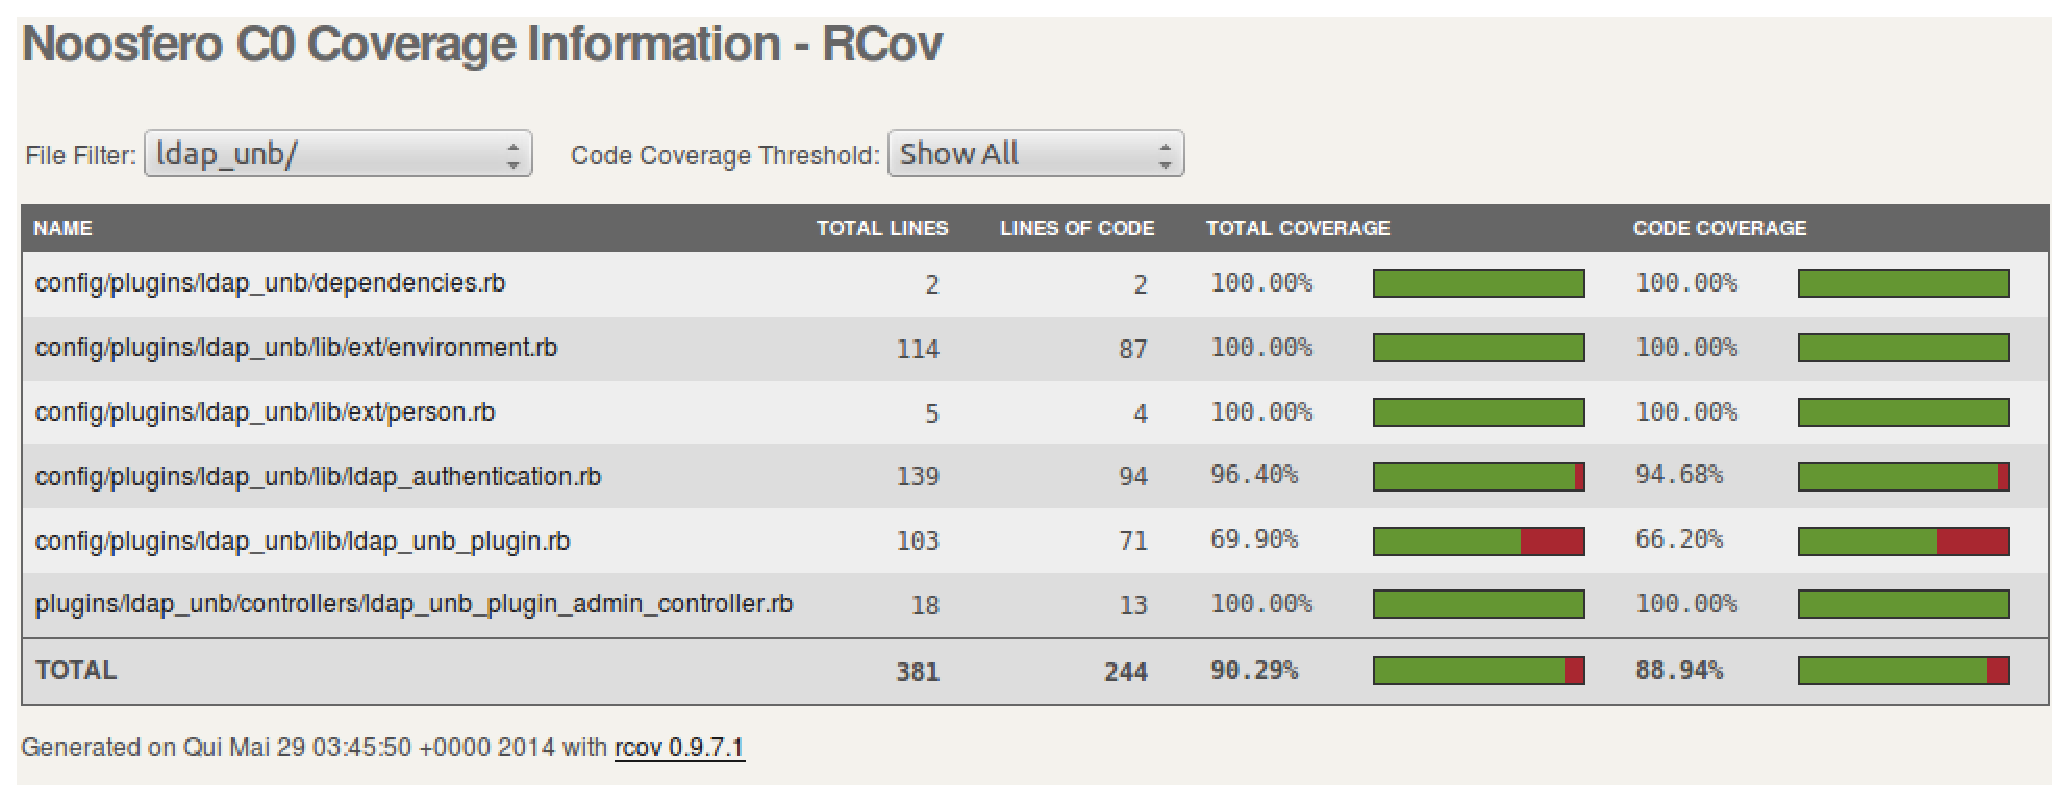
\includegraphics[keepaspectratio=false,scale=0.45]
      {images/cobertura_teste.eps}
    \caption{Cobertura de código do plugin LdapUnb}
    \label{consideracoes_cobertura1}
\end{figure}

Outro \textit{plugin} (plugin de Envio de TCC) desenvolvido para o Noosfero, porém em uma aplicação diferente, o Portal UnB Gama, é responsável por criar uma atribuição de trabalhos, chamada de \textit{work assignment}. Essa atribuição possui algumas funcionalidades específicas como possibilitar que os usuários envolvidos sejam notificados via \textit{email} sobre a submissão de um certo trabalho. Segue os dados sobre a execução dos testes funcionais e unitários:

\begin{itemize}
\item Quantidade de testes executados: \textbf{28 testes};
\item Quantidade de assertivas executadas: \textbf{84 assertivas};
\item Quantiadde de falhas obtidas: \textbf{0 falhas};
\item Tempo de execução dos testes: \textbf{10,5 segundos};
\end{itemize}

Na imagem \ref{consideracoes_cobertura2} está representado a cobertura de código, extraída da ferramenta Rcov:

\begin{figure}[!h]
    \centering
    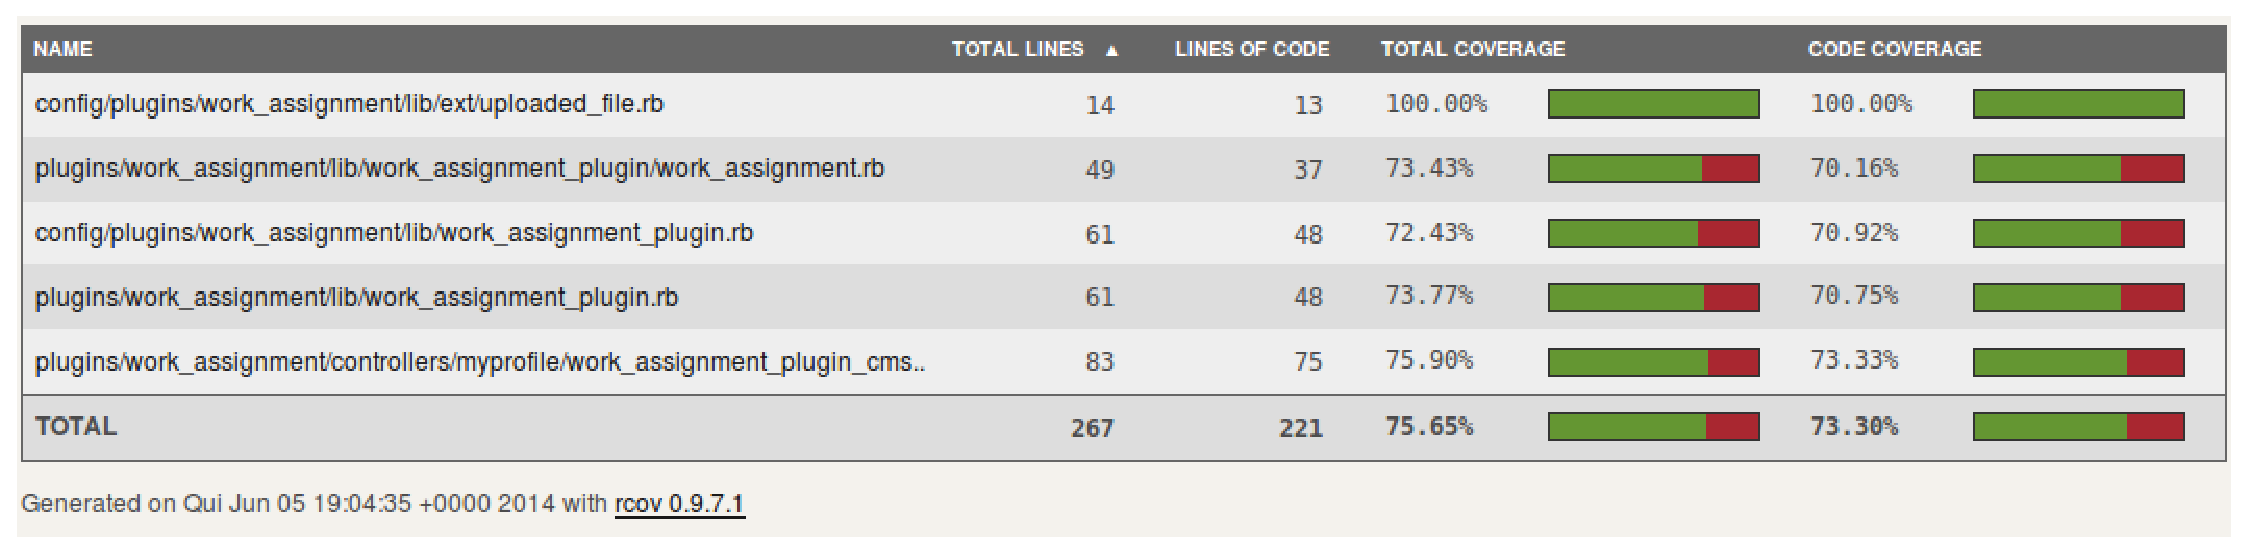
\includegraphics[keepaspectratio=false,scale=0.45]
      {images/cobertura_tcc.eps}
    \caption{Cobertura de código do plugin para submissão de trabalho}
    \label{consideracoes_cobertura2}
\end{figure}

Para o plugin de envio de tcc, foram definidos testes de aceitação, para verificar o comportamento da funcionalidade que foi desenvolvida, obtendo os seguintes dados:

\begin{itemize}
\item Quantidade de cenários executados: \textbf{6 cenários};
\item Quantidade de passos executadas: \textbf{130 passos};
\item Quantiadde de falhas obtidas: \textbf{0 falhas};
\item Tempo de execução dos testes: \textbf{7 minutos e 18 segundos};
\end{itemize}

A partir do desenvolvimento dos plugins verificamos que a utilização de práticas de TDD e BDD como base para o desenvolvimento trouxe resultados satisfatórios. Com a proposta de algumas técnicas de avaliação da usabilidade para o Portal da Participação Social, verificamos que muitas delas precisam ser adaptadas para uma melhor adoção nos ambientes de software livre.
